\documentclass[12pt,openright,a4paper]{report}
\usepackage[utf8]{inputenc}
\usepackage[brazil]{babel}
\usepackage{amsfonts,amssymb,graphicx,enumerate}
\usepackage[centertags]{amsmath}
% Configuracoes de pagina
\usepackage[lmargin=3cm,rmargin=3cm,tmargin=3cm,bmargin=3cm]{geometry}
% Layout da pagina
\usepackage{hyperref}
% Layout para código
\usepackage{listings}
% Font for code style
\usepackage{courier}
% The 68 standard colors known to dvips
\usepackage[usenames,dvipsnames]{xcolor}
\hypersetup{pdfpagelayout= SinglePage,
    colorlinks=true,
	linkcolor=blue,          	% color of internal links
    pdftitle={Relatório de Redes},
    pdfauthor={Áulus Diniz, Arthur Jahn, Gabriel Araújo, Jonatas Lenon}}

%*******************************************************
\definecolor{light-gray}{gray}{0.90}
\lstset{
  backgroundcolor=\color{light-gray},
  basicstyle=\footnotesize\ttfamily,
  breaklines=true
}

\frenchspacing 

\title{Fundamentos de Redes de Computadores: \\ Servidor DNS com Extensões DNSSEC}
\author{Arthur Jahn, Áulus Diniz, Gabriel Araújo, Jonatas Lenon}
\date{26 de Novembro de 2015}    %para ocultar a data digite: \date{ }
%*******************************************************
\begin{document}    %Inicio do documento
\maketitle  %cria o titulo na capa

\pagebreak

\tableofcontents %Sumario
%-------------------------------------------------------
\chapter{Problema e Motivação}
\label{chap_problema}

O DNS provê serviços de resolução de \textit{hosts} por meio da tradução de nomes de domínios em números de endereçamento IP. Como um mesmo domínio pode estar vinculado a vários endereços IP, esse serviço pode ser responsável também por distribuição de carga entre os \textit{hosts} de destino, alternando o endereço fornecido ao cliente quando uma solicitação de resolução de domínio é feita.\\

Quando o DNS foi projetado, no início dos anos 80, não foram pensadas questões de segurança. No momento de uma requisição DNS, o cliente simplesmente confia que a informação recebida é válida e legítima. Essa forma de requisição cria vulnerabilidades com o envenenamento de \textit{cache}.\\

Para se corigir tais vulnerabilidades, foram definidas extensões de segurança para prover confiabilidade nos registros trocados via DNS: o DNSSEC. Para que não fosse modificada a forma como o DNS opera, o DNSSEC simplemente adiciona novos tipos de registros ao DNS como o RRSIG e o DNSKEY e podem ser requisitados da mesma forma como registros do tipo A, CNAME ou MX.\\

Neste trabalho, pretende-se apresentar como configurar um DNS com as extensões de segurança segundo o DNSSEC e apresentar o passo-a-passo para que um cliente faça requisições seguras. O processo como um todo para configuração das ferramentas utilizadas e como executar o sistema é apresentado a seguir.

\chapter{DNS  - \textit{Domain Name System}}
\label{chap_dns}

Uma consulta DNS comum consiste basicamente de uma requisição enviada pelo cliente seguida de uma resposta devolvida pelo servidor. Nesse sentido, é interessante a utilização de um protocolo de transporte sem estabelecimento de conexão como o UDP para não acarretar em um atraso na requisição, como no caso do protocolo TCP que necessita de um \textit{handshake} de três vias. O processo para configuração do servidor DNS utilizado neste trabalho está descrito a seguir.

\section{Configuração do Servidor DNS}
\label{sec_configuracao}

O servido DNS utilizado nesse experimento foi o Bind9 - \textit{Berkeley Internet Name Domain} - comumente encontrado em distribuições linux.

Para a instalação do servidor Bind, caso não esteja instalado, pode-se instalar seguindo o seguinte passo:

\begin{lstlisting}[language=bash]

	sudo apt-get install bind9 dnsutils

\end{lstlisting}

Após a instalação do servidor DNS é necessario configurar as zonas de endereçamento. Cada zona consiste em um mapeamento de uma URL para um endereço de IP e vice-versa. Para configurar uma zona no Bind, deve-se criar uma arquivo de zona.

Navegue até a pasta referente ao servidor Bind e crie uma pasta para armazenar os arquivos de zona.

\begin{lstlisting}[language=bash]

	cd /etc/bind

	mkdir -p zones/master

\end{lstlisting}

O arquivo de zona criado é referênte ao site www.tcpdump.org. Portando o nome do arquivo deve ser: \textit{db.tcpdump.org} e deve conter o seguinte conteudo:

\begin{lstlisting}[language=bash]

;
; BIND data file for tcpdump.org
;
$TTL    3h
@       IN      SOA     ns1.tcpdump.org. admin.tcpdump.org. (
                          1        ; Serial
                          3h       ; Refresh after 3 hours
                          1h       ; Retry after 1 hour
                          1w       ; Expire after 1 week
                          1h )     ; Negative caching TTL of 1 day
;
@       IN      NS      ns1.tcpdump.org.
@       IN      NS      ns2.tcpdump.org.


tcpdump.org.    IN      MX      10      mail.tcpdump.org.
tcpdump.org.    IN      A       192.139.46.66
ns1                     IN      A       192.139.46.66
ns2                     IN      A       192.139.46.66
www                     IN      CNAME   tcpdump.org.
mail                    IN      A       192.139.46.66
ftp                     IN      CNAME   tcpdump.org.

\end{lstlisting}

Com o arquivo de zona configurado é necessário informar ao ao servidor DNS a localização desse arquivo.

\begin{lstlisting}[language=bash]
zone "tcpdump.org" {
       type master;
       file "/etc/bind/zones/master/db.linuxconfig.org";
};
\end{lstlisting}

Com esses arquivos é possivel a partir de uma URL descobrir seu IP.

Uma última coisa é adicionar um endereço de IP de um servidor DNS estável no arquivo named.conf.options. Este endereço de IP é usado quando o servidor DNS local não sabe a resposta para a consulta de resolução de nome. Para este experimento foi utilizado o servidor de DNS do google - 8.8.8.8 ou 8.8.4.4.

\begin{lstlisting}[language=bash]
 forwarders {
     8.8.4.4;
};
\end{lstlisting}

Com as configurações realizadas liga-se o servidor Bind da seguinte forma:

\begin{lstlisting}[language=bash]
 cd /etc/init.d/
 sudo ./bind9 start
\end{lstlisting}

Com os servidor DNS Bind é possivel obter o endereço de IP de um site através de um requisição, utilizando o comando dig, no servidor DNS local. Nesse experimento o IP da máquina com o servidor DNS é: 192.168.1.23

\begin{lstlisting}[language=bash]
 dig @192.168.1.23 tcpdump.org

 ; <<>> DiG 9.8.3-P1 <<>> @192.168.1.23 tcpdump.org
; (1 server found)
;; global options: +cmd
;; Got answer:
;; ->>HEADER<<- opcode: QUERY, status: NOERROR, id: 30817
;; flags: qr aa rd ra; QUERY: 1, ANSWER: 1, AUTHORITY: 2, ADDITIONAL: 2

;; QUESTION SECTION:
;tcpdump.org.			IN	A

;; ANSWER SECTION:
tcpdump.org.		10800	IN	A	192.139.46.66

;; AUTHORITY SECTION:
tcpdump.org.		10800	IN	NS	ns1.tcpdump.org.
tcpdump.org.		10800	IN	NS	ns2.tcpdump.org.

;; ADDITIONAL SECTION:
ns1.tcpdump.org.	10800	IN	A	192.139.46.66
ns2.tcpdump.org.	10800	IN	A	192.139.46.66

;; Query time: 165 msec
;; SERVER: 192.168.1.23#53(192.168.1.23)
;; WHEN: Sat Nov 14 16:18:10 2015
;; MSG SIZE  rcvd: 113
\end{lstlisting}

\section{Vulnerabilidades}
\label{sec_vulnerabilidades}

Com a utilização de protocolo UDP, como não há estabelecimento de conexão apenas um QID (i.e. \textit{query ID}), um atacante pode tentar utilizar vários pacotes para simular respostas de um servidor DNS conhecido e eventualmente enviar um pacote com um QID válido para o cliente. Nesse momento, o atacante conseguirá inserir no \textit{cache} do cliente um redirecionamento de uma página conhecida para uma outra controlada por ele. Essa é apenas uma vulnerabilidade conhecida como envenenamento de \textit{cahe}. Esse e outros tipos de ataques são melhor explicados a seguir.\\

{\textbf{Envenenamento de Cache (Cache Poisoning):} este é um dos mais conhecidos e difundidos ataques a segurança do DNS, ocorrendo quando um cliente realiza uma consulta para um determinado dominio, esta consulta é feita a uma zona DNS, porém esta zona não é fornecida por um servidor autoritativo os quais possuem os registros originais que associam aquele domínio a seu endereço de IP, assim um outro servidor de Cache DNS que encontra-se configurado nos resolvers do computador do cliente responde primeiro a requisição do cliente, levando o este a um servidor que não é o servidor de origem dodomínio, assim fornecendo informações forjadas ao cliente. Este cenario é comumente utilizado para levar o utilizador as denominadas páginas de Phishing, onde os dados submetidos pelo resolver são capturadas pelo hacker.\\

\textbf{ Ataque de negação de serviço ou DDoS (Distributed Denial of Service): }Acontece quando um invasor tenta negar a disponibilidade de serviços DNS, através de consultas recursivas, consumindo todos os recursos como memória e processador do servidor, tornando-o indisponível.\\

\textbf{ Modificação de dados: } Após ocupar uma rede usando DNS, O invasor tenta usar os endereços IP válidos, em pacotes IP criados pelo invasor, assim esses pacotes passam a ter a aparência de um endereço IP válido na rede. Normalmente isso é denominado falsificação de IP.\\

\textbf{ man-in-the-middle (Homem no meio): } Nesse ataque, os dados trocados entre duas partes são interceptados, e assim essas informações são registrados e possivelmente alteradas pelo atacante, sem que as vítimas tomem conhecimento dessa ação, fazendo com que os envolvidos acreditem que estão se comunicando diretamente em uma conexão privada, quando de fato a conversa é controlada pelo atacante.

\chapter{ DNSSEC  - \textit{Domain Name System Security Extensions}}
\label{chap_dnssec}

O DNSSEC é uma solução que expande a segurança do serviço DNS, permitindo validar a origem dos dados, assegurar que a informação recebida de um servidor DNS é autêntica, confirmando que a informação não foi alterada durante a passagem pelos vários “nodos” da Internet e confirmar a inexistência de um domínio.\\

O sistema DNSSEC introduz apenas alguns novos tipos de Registos nas zonas DNS, nomeadamente DNSKEY, RRSIG e DS, sendo compatível com servidores ou clientes que não tenham implementado o DNSSEC. As extensões de segurança DNSSEC utilizam criptografia assimétrica, permitindo que a verificação e troca de informação DNS entre o servidor e o cliente seja privada e entregue sem alterações, recorrendo a uma assinatura digital e um conjunto de chaves privadas e publicas.\\

O DNSSEC é baseado numa cadeia de confiança, onde inicialmente é validada a raiz “.”, assinada digitalmente pela ICANN e IANA. Posteriormente a raiz assina a zona “.pt” utilizando a sua chave privada e anexa-lhe a chave publica, permitindo a partir desse momento que quando um servidor de nomes local fizer uma consulta relacionada com um domínio “.pt”, este possa validar a autenticidade da raiz “.pt” recorrendo à chave publica. O processo é repetido, até chegar à zona final correspondente ao domínio que está a ser assinado e validado. As extensões de segurança do DNS são totalmente compatíveis com IPv6, uma vez que apenas é validada a integridade dos registos.

\section{Configuração do Servidor DNS Seguro}
\label{sec_config_segura}

\section{Configuração do Servidor DNS Seguro}
\label{sec_config_segura}

\textbf{DNSSEC Resource Records}
\\\ Um \textit{ Resource Records(RR)} contém uma informação específica sobre o domínio. Alguns dos mais comuns são registro que contém o endereço IP do domínio, registros AAAA que detém as informações IPv6, e também os registro MX contendo servidores de e-mail. O DNSSEC contém várias RRS, as quais destacam-se:

\begin{itemize}
\item \textbf{DNSKEY} contém a chave pública que os resolvers utilizam para validar a conexão.
\item \textbf{RRSIG} existe para cada RR e contém a assinatura digital de um registro.
\item \textbf{DS \textit{(Delegation Signer)}} - este registro existe em \textit{TLD's nameservers}. O objetivo desse registro é verificar a autenticidade do próprio DNSKEY.
\end{itemize}

\textbf{Domain Name}: redesfga.com

\textbf{Master Nameserver:} Endereço IP: 1.1.1.1 Hostname: master.redesfga.com OS: Ubuntu 14\\

\textbf{Master}: Debian\\

\textbf{Nome do serviço}: Bind9\\

Abra os seguintes arquivos:

- Configuração principal
\begin{lstlisting}[language=bash]
	/etc/bind/named.conf.options
\end{lstlisting}

- Arquivo nomes Zona
\begin{lstlisting}[language=bash]
	/etc/bind/named.conf.local
\end{lstlisting}

- Arquivo de zona Padrão
\begin{lstlisting}[language=bash]
	/var/cache/bind/	
\end{lstlisting}

\subsection{Configuração do DNSSec Master}
Ative o DNSSEC adicionando as seguintes diretivas de configuração dentro de options{ }
\begin{lstlisting}[language=bash]
	nano /etc/bind/named.conf.options
	
	dnssec-enable yes;
	dnssec-validation yes;
	dnssec-lookaside auto;
\end{lstlisting}

Navegue até seus arquivos de zona.
\begin{lstlisting}[language=bash]
	cd /var/cache/bind	
\end{lstlisting}

Crie uma chave de assinatura de zona \textit{Zone Signing Key(ZSK)} com este comando
\begin{lstlisting}[language=bash]
	dnssec-keygen -a NSEC3RSASHA1 -b 2048 -n ZONE redesfga.com
\end{lstlisting}

Intale o \textbf{haveged} para a criação da chave mais rápidamente
\begin{lstlisting}[language=bash]
	sudo apt-get install haveged
\end{lstlisting}

Crie uma \textit{Key Signing Key(KSK)}.
\begin{lstlisting}[language=bash]
	dnssec-keygen -f KSK -a NSEC3RSASHA1 -b 4096 -n ZONE redesfga.com
\end{lstlisting}

A saida do terminal deve ser semelhante ao exemplo a seguir:
\begin{lstlisting}[language=bash]
	root@master:/var/cache/bind# dnssec-keygen -f KSK -a NSEC3RSASHA1 -b 4096 -n ZONE redesfga.com
	Generating key pair......................++ 			...........................................................................		++
	Kredesfga.com.+007+62910	
\end{lstlisting}

O diretório agora terá 4 chaves - pares de chaves privadas e publicas de ZSK e KSK. É necessário adicionar a chave publica que contém o registro \textbf{DNSKEY} para o arquivo de zona.

A estrutura \textit{for} seguinte deve realizar esta tarefa:
\begin{lstlisting}[language=bash]
	for key in `ls Kredesfga.com*.key`
	do
	echo "\$INCLUDE $key">> db.redesfga.com
	done
\end{lstlisting}

Agora a zona deve ser assinada usando o comando:
\begin{lstlisting}[language=bash]
	dnssec-signzone -3 <salt> -A -N INCREMENT -o <zonename> -t <zonefilename>
\end{lstlisting}

Utilize um \textit{salt} diferente. O comando deve gerar a seguinte saída:
\begin{lstlisting}[language=bash]
	root@master:/var/cache/bind# dnssec-signzone -A -3 $(head -c 1000 /dev/random | sha1sum | cut -b 1-16) -N 	INCREMENT -o redesfga.com -t db.redesfga.com
	Verifying the zone using the following algorithms: NSEC3RSASHA1.
	Zone signing complete:
	Algorithm: NSEC3RSASHA1: KSKs: 1 active, 0 stand-by, 0 revoked
    	                    ZSKs: 1 active, 0 stand-by, 0 revoked
	example.com.zone.signed
	Signatures generated:                       14
	Signatures retained:                         0
	Signatures dropped:                          0
	Signatures successfully verified:            0
	Signatures unsuccessfully verified:          0
	Signing time in seconds:                 0.046
	Signatures per second:                 298.310
	Runtime in seconds:                      0.056

\end{lstlisting}

Uma string de 16 caracteres pode ser gerada para salt usando o comando:
\begin{lstlisting}[language=bash]
	head -c 1000 /dev/random | sha1sum | cut -b 1-16
\end{lstlisting}

Isto cria um arquivo chamado db.redesfga.com.signed que contém o registro \textbf{RRSIG} para cada registro DNS. Agora é necessário avisar o BIND para carregar a zona 'assinada'.
\begin{lstlisting}[language=bash]
	nano /etc/bind/named.conf.local
\end{lstlisting}

Mude a opção \textbf{file} dentro da seção \textbf{"zone \{ \}" }.
\begin{lstlisting}[language=bash]
	zone "redesfga.com" IN {
	    type master;
	    file "db.redesfga.com.signed";
	    allow-transfer { 2.2.2.2; };
    	allow-update { none; };
	};
\end{lstlisting}

Após salvar o arquivo recarregue o serviço do \textbf{bind}.
\begin{lstlisting}[language=bash]
	nano /etc/bind/named.conf.local
\end{lstlisting}

\begin{lstlisting}[language=bash]
	service bind9 reload
\end{lstlisting}

Verifique pelo registro de DNSKEY usando o comando \textbf{dig} no mesmo servidor.
\begin{lstlisting}[language=bash]
	dig DNSKEY redesfga.com. @localhost +multiline
\end{lstlisting}

O comando deve gerar a seguinte saída:
\begin{lstlisting}[language=bash]
root@master:/var/cache/bind# dig DNSKEY example.com. @localhost +multiline
;; Truncated, retrying in TCP mode.

; <<>> DiG 9.8.4-rpz2+rl005.12-P1 <<>> DNSKEY example.com. @localhost +multiline
;; global options: +cmd
;; Got answer:
;; ->>HEADER<<- opcode: QUERY, status: NOERROR, id: 43986
;; flags: qr aa rd; QUERY: 1, ANSWER: 2, AUTHORITY: 0, ADDITIONAL: 0
;; WARNING: recursion requested but not available

;; QUESTION SECTION:
;example.com.       IN DNSKEY

;; ANSWER SECTION:
redesfga.com.        86400 IN DNSKEY   256 3 7 (
                AwEAActPMYurNEyhUgHjPctbLCI1VuSj3xcjI8QFTpdM
                8k3cYrfwB/WlNKjnnjt98nPmHv6frnuvs2LKIvvGzz++
                kVwVc8uMLVyLOxVeKhygDurFQpLNNdPumuc2MMRvV9me
                fPrdKWtEEtOxq6Pce3DW2qRLjyE1n1oEq44gixn6hjgo
                sG2FzV4fTQdxdYCzlYjsaZwy0Kww4HpIaozGNjoDQVI/
                f3JtLpE1MYEb9DiUVMjkwVR5yH2UhJwZH6VVvDOZg6u6
                YPOSUDVvyofCGcICLqUOG+qITYVucyIWgZtHZUb49dpG
                aJTAdVKlOTbYV9sbmHNuMuGt+1/rc+StsjTPTHU=
                ) ; key id = 40400
redesfga.com.        86400 IN DNSKEY   257 3 7 (
                AwEAAa2BE0dAvMs0pe2f+D6HaCyiFSHw47BA82YGs7Sj
                qSqH3MprNra9/4S0aV6SSqHM3iYZt5NRQNTNTRzkE18e
                3j9AGV8JA+xbEow74n0eu33phoxq7rOpd/N1GpCrxUsG
                kK4PDkm+R0hhfufe1ZOSoiZUV7y8OVGFB+cmaVb7sYqB
                RxeWPi1Z6Fj1/5oKwB6Zqbs7s7pmxl/GcjTvdQkMFtOQ
                AFGqaaSxVrisjq7H3nUj4hJIJ+SStZ59qfW3rO7+Eqgo
                1aDYaz+jFHZ+nTc/os4Z51eMWsZPYRnPRJG2EjJmkBrJ
                huZ9x0qnjEjUPAcUgMVqTo3hkRv0D24I10LAVQLETuw/
                QOuWMG1VjybzLbXi5YScwcBDAgtEpsQA9o7u6VC00DGh
                +2+4RmgrQ7mQ5A9MwhglVPaNXKuI6sEGlWripgTwm425
                JFv2tGHROS55Hxx06A416MtxBpSEaPMYUs6jSIyf9cjB
                BMV24OjkCxdz29zi+OyUyHwirW51BFSaOQuzaRiOsovM
                NSEgKWLwzwsQ5cVJBEMw89c2V0sHa4yuI5rr79msRgZT
                KCD7wa1Hyp7s/r+ylHhjpqrZwViOPU7tAGZ3IkkJ2SMI
                e/h+FGiwXXhr769EHbVE/PqvdbpcsgsDqFu0K2oqY70u
                SxnsLB8uVKYlzjG+UIoQzefBluQl
                ) ; key id = 62910

;; Query time: 0 msec
;; SERVER: 127.0.0.1#53(127.0.0.1)
;; WHEN: Wed Nov 27 18:18:30 2013
;; MSG SIZE  rcvd: 839

Check for the presence of RRSIG records.

dig A redesfga.com. @localhost +noadditional +dnssec +multiline
; <<>> DiG 9.8.4-rpz2+rl005.12-P1 <<>> A redesfga.com. @localhost +noadditional +dnssec +multiline
;; global options: +cmd
;; Got answer:
;; ->>HEADER<<- opcode: QUERY, status: NOERROR, id: 32902
;; flags: qr aa rd; QUERY: 1, ANSWER: 2, AUTHORITY: 3, ADDITIONAL: 5
;; WARNING: recursion requested but not available

;; OPT PSEUDOSECTION:
; EDNS: version: 0, flags: do; udp: 4096
;; QUESTION SECTION:
;redesfga.com.         IN A

;; ANSWER SECTION:
redesfga.com.          86400 IN A 93.184.216.119
redesfga.com.          86400 IN RRSIG A 7 2 86400 20131227171405 (
                            20131127171405 40400 example.com.
                            JCoL8L7As1a8CXnx1W62O94eQl6zvVQ3prtNK7BWIW9O
                            lir/4V+a6c+0tbt4z4lhgmb0sb+qdvqRnlI7CydaSZDb
                            hlrJA93fHqFqNXw084YD1gWC+M8m3ewbobiZgBUh5W66
                            1hsVjWZGvvQL+HmobuSvsF8WBMAFgJgYLg0YzBAvwHIk
                            886be6vbNeAltvPl9I+tjllXkMK5dReMH40ulgKo+Cwb
                            xNQ+RfHhCQIwKgyvL1JGuHB125rdEQEVnMy26bDcC9R+
                            qJNYj751CEUZxEEGI9cZkD44oHwDvPgF16hpNZGUdo8P
                            GtuH4JwP3hDIpNtGTsQrFWYWL5pUuuQRwA== )

;; AUTHORITY SECTION:
redesfga.com.          86400 IN NS master.example.com.
redesfga.com.          86400 IN RRSIG NS 7 2 86400 20131227171405 (
                            20131127171405 40400 example.com.
                            hEGzNvKnc3sXkiQKo9/+ylU5WSFWudbUc3PAZvFMjyRA
                            j7dzcVwM5oArK5eXJ8/77CxL3rfwGvi4LJzPQjw2xvDI
                            oVKei2GJNYekU38XUwzSMrA9hnkremX/KoT4Wd0K1NPy
                            giaBgyyGR+PT3jIP95Ud6J0YS3+zg60Zmr9iQPBifH3p
                            QrvvY3OjXWYL1FKBK9+rJcwzlsSslbmj8ndL1OBKPEX3
                            psSwneMAE4PqSgbcWtGlzySdmJLKqbI1oB+d3I3bVWRJ
                            4F6CpIRRCb53pqLvxWQw/NXyVefNTX8CwOb/uanCCMH8
                            wTYkCS3APl/hu20Y4R5f6xyt8JZx3zkZEQ== )

;; Query time: 0 msec
;; SERVER: 127.0.0.1#53(127.0.0.1)
;; WHEN: Thu Nov 28 00:01:06 2013
;; MSG SIZE  rcvd: 1335
\end{lstlisting}

E então a configuração do servidor master está completa.

\section{Requisições seguras}
\label{sec_req_seguras}

Cada zona no DNSSEC tem um par de assinatura de chave(ZSK): a parte privada da chave assina digitalmente cada RRset na zona, enquanto que a porção pública verifica a assinatura. Para habilitar o DNSSEC, um operador de zona cria assinaturas digitais para cada RRset usando o ZSK privado e os armazena em seu servidor DNS como registros RRSIG. Isso é como dizer: "Estes são os meus registros de DNS, eles vêm do meu servidor, e eles devem ser assim", como mostra a figura \ref{fig:keys}.

\begin{figure}[h!]
	\centering
	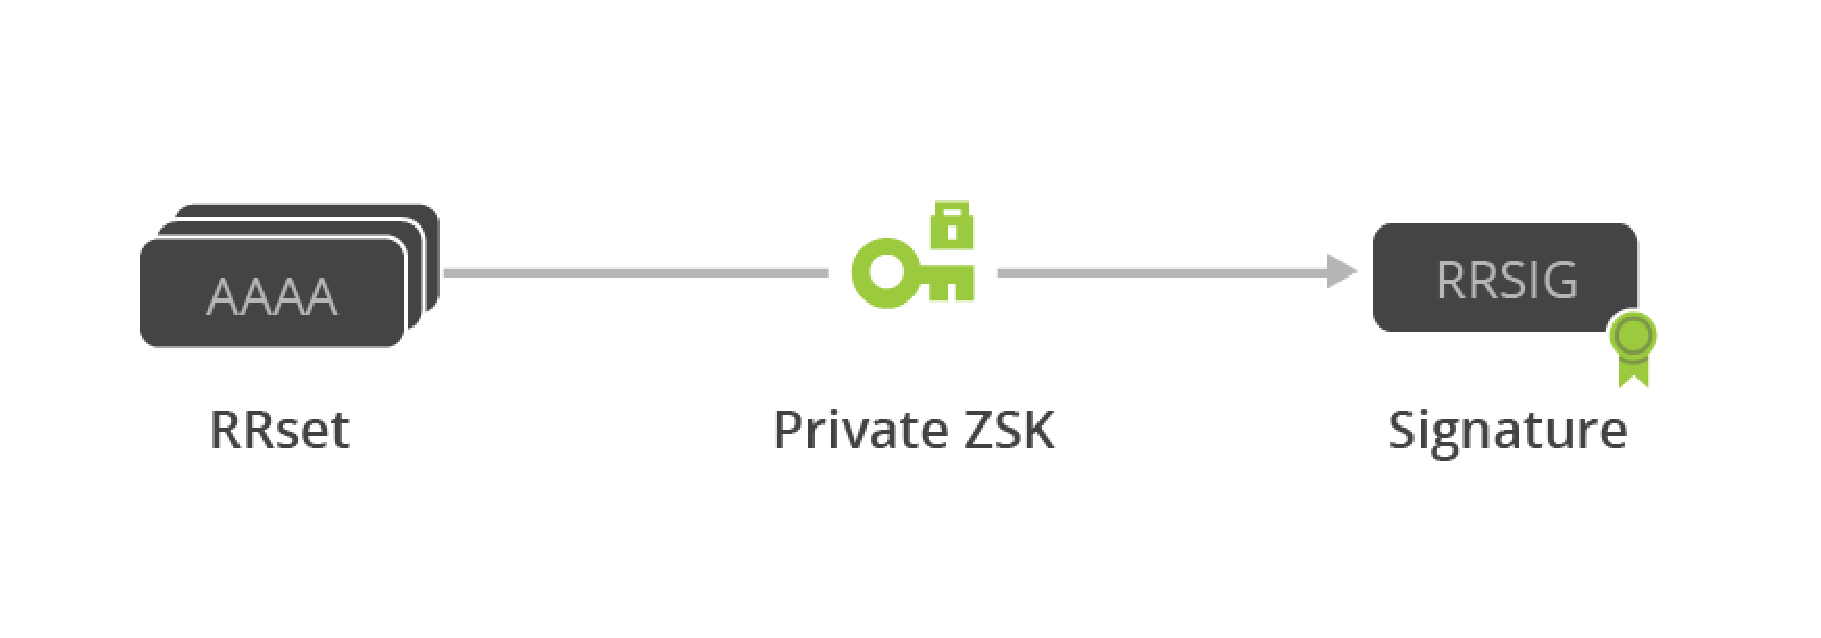
\includegraphics[scale=0.4]{keys.eps}
	\caption{Chave de assinatura para RRSet.}
	\label{fig:keys}
\end{figure}

Quando um cliente DNSSEC solicita um tipo de registro em particular (por exemplo, AAAA), o servidor DNS também retorna o RRSIG correspondente. O cliente pode em seguida puxar o registro DNSKEY contendo a ZSK pública a partir do servidor de nomes. Juntos, o RRset, RRSIG, e ZSK público podem validar a resposta.

\begin{figure}[h!]
	\centering
	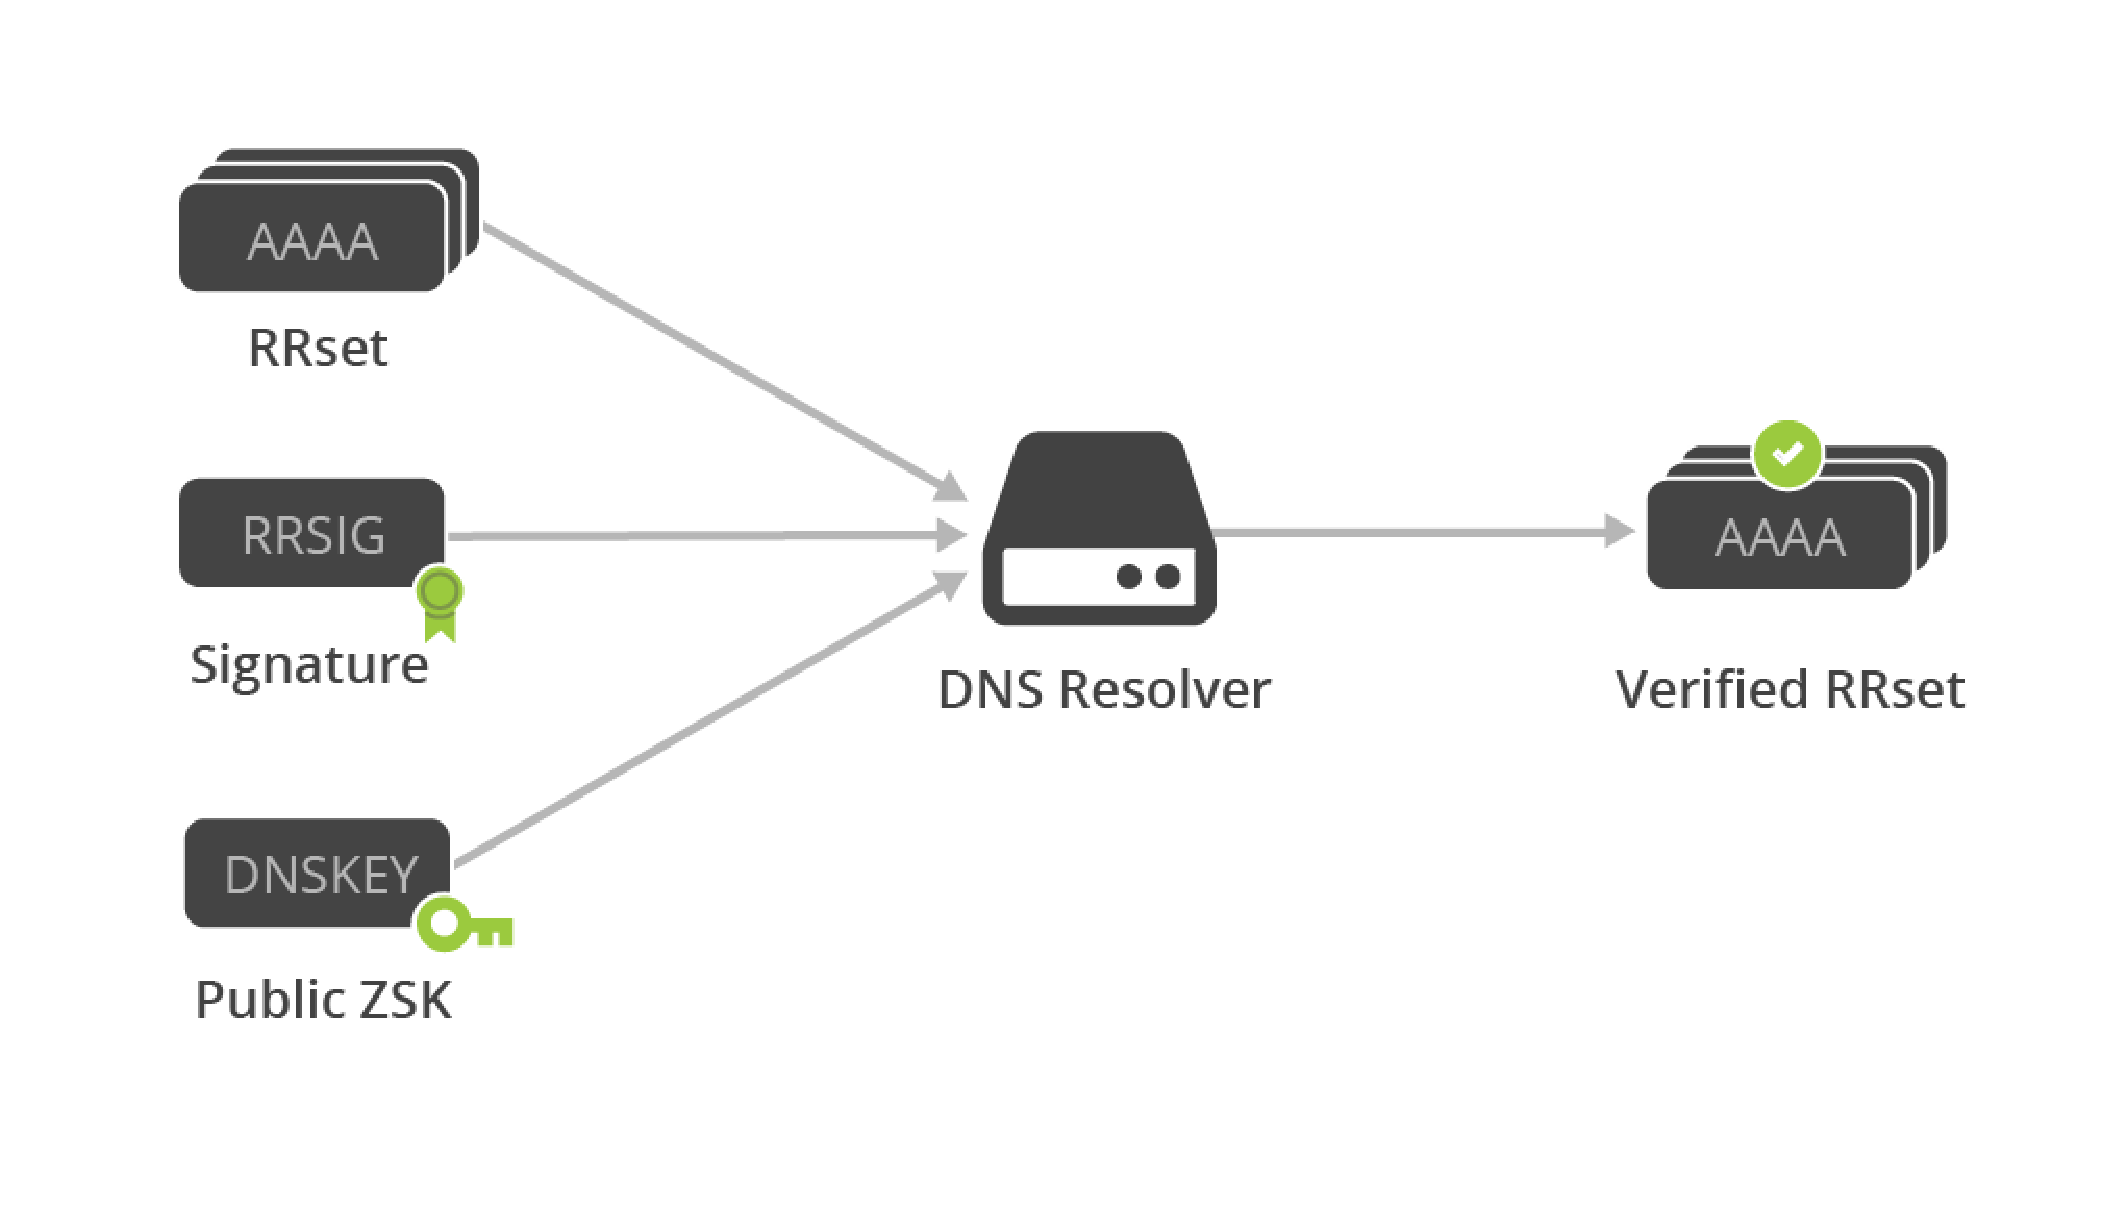
\includegraphics[scale=0.4]{validation.eps}
	\caption{Validação de registros RRSIG.}
	\label{fig:keys}
\end{figure}

Precisa-se de uma forma de validar a ZSK pública, uma vez que não se sabe se houve alteração. Para isso, verifica-se a "validade da validade". 

Além de uma chave de assinatura de zona, servidores DNSSEC também possuem uma chave de assinatura (KSK). O KSK valida o registro DNSKEY exatamente da mesma maneira como nosso ZSK garantiu o resto de nossas RRsets na seção anterior: Ele assina a ZSK público (que é armazenado em um registro DNSKEY), criando uma RRSIG para o DNSKEY.

\begin{figure}[h!]
	\centering
	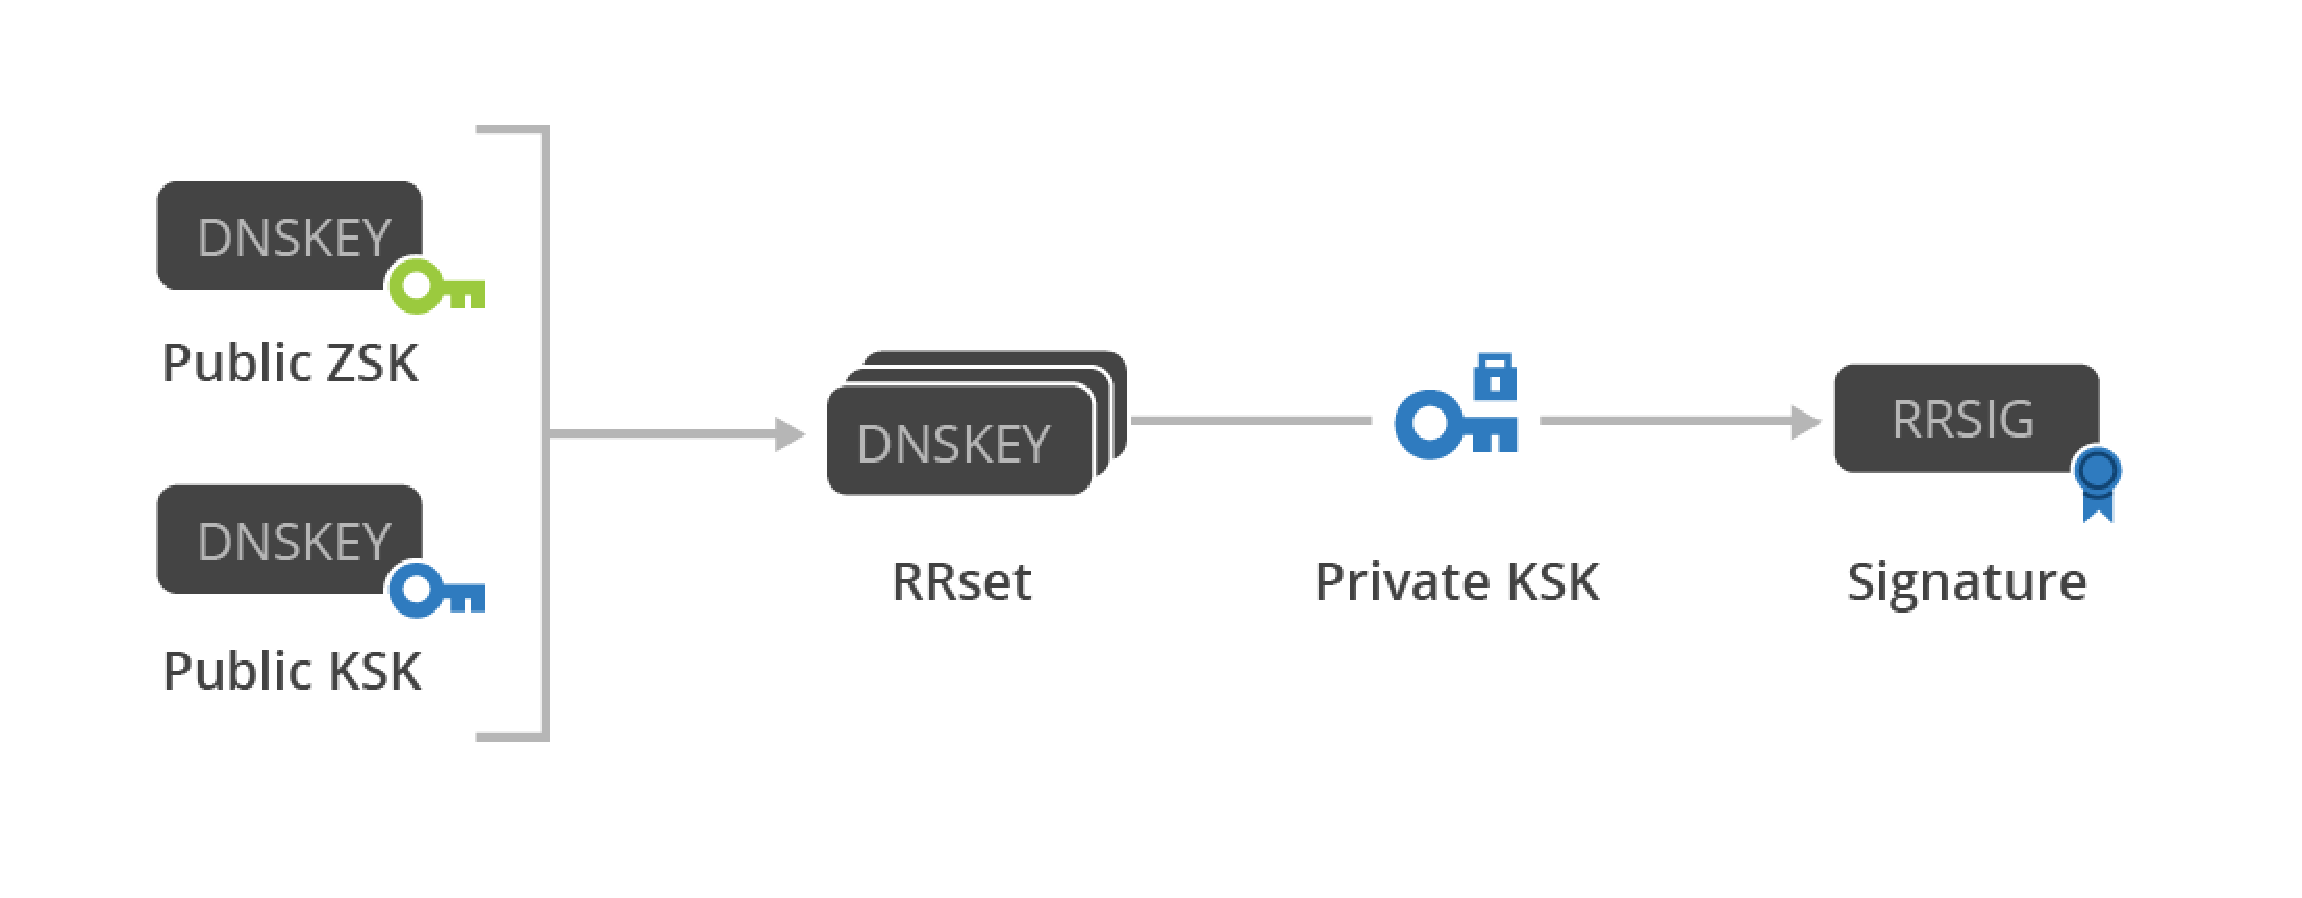
\includegraphics[scale=0.4]{valid_validation.eps}
	\caption{Verificação da validade da chave.}
	\label{fig:keys}
\end{figure}

Assim como o ZSK público, o servidor de nomes publica o KSK pública em outro registro DNSKEY, que nos dá a RRset DNSKEY mostrado acima. Tanto o KSK e ZSK pública público são assinados pelo KSK privada. Clientes pode então utilizar a KSK pública para validar a ZSK pública.

\begin{figure}[h!]
	\centering
	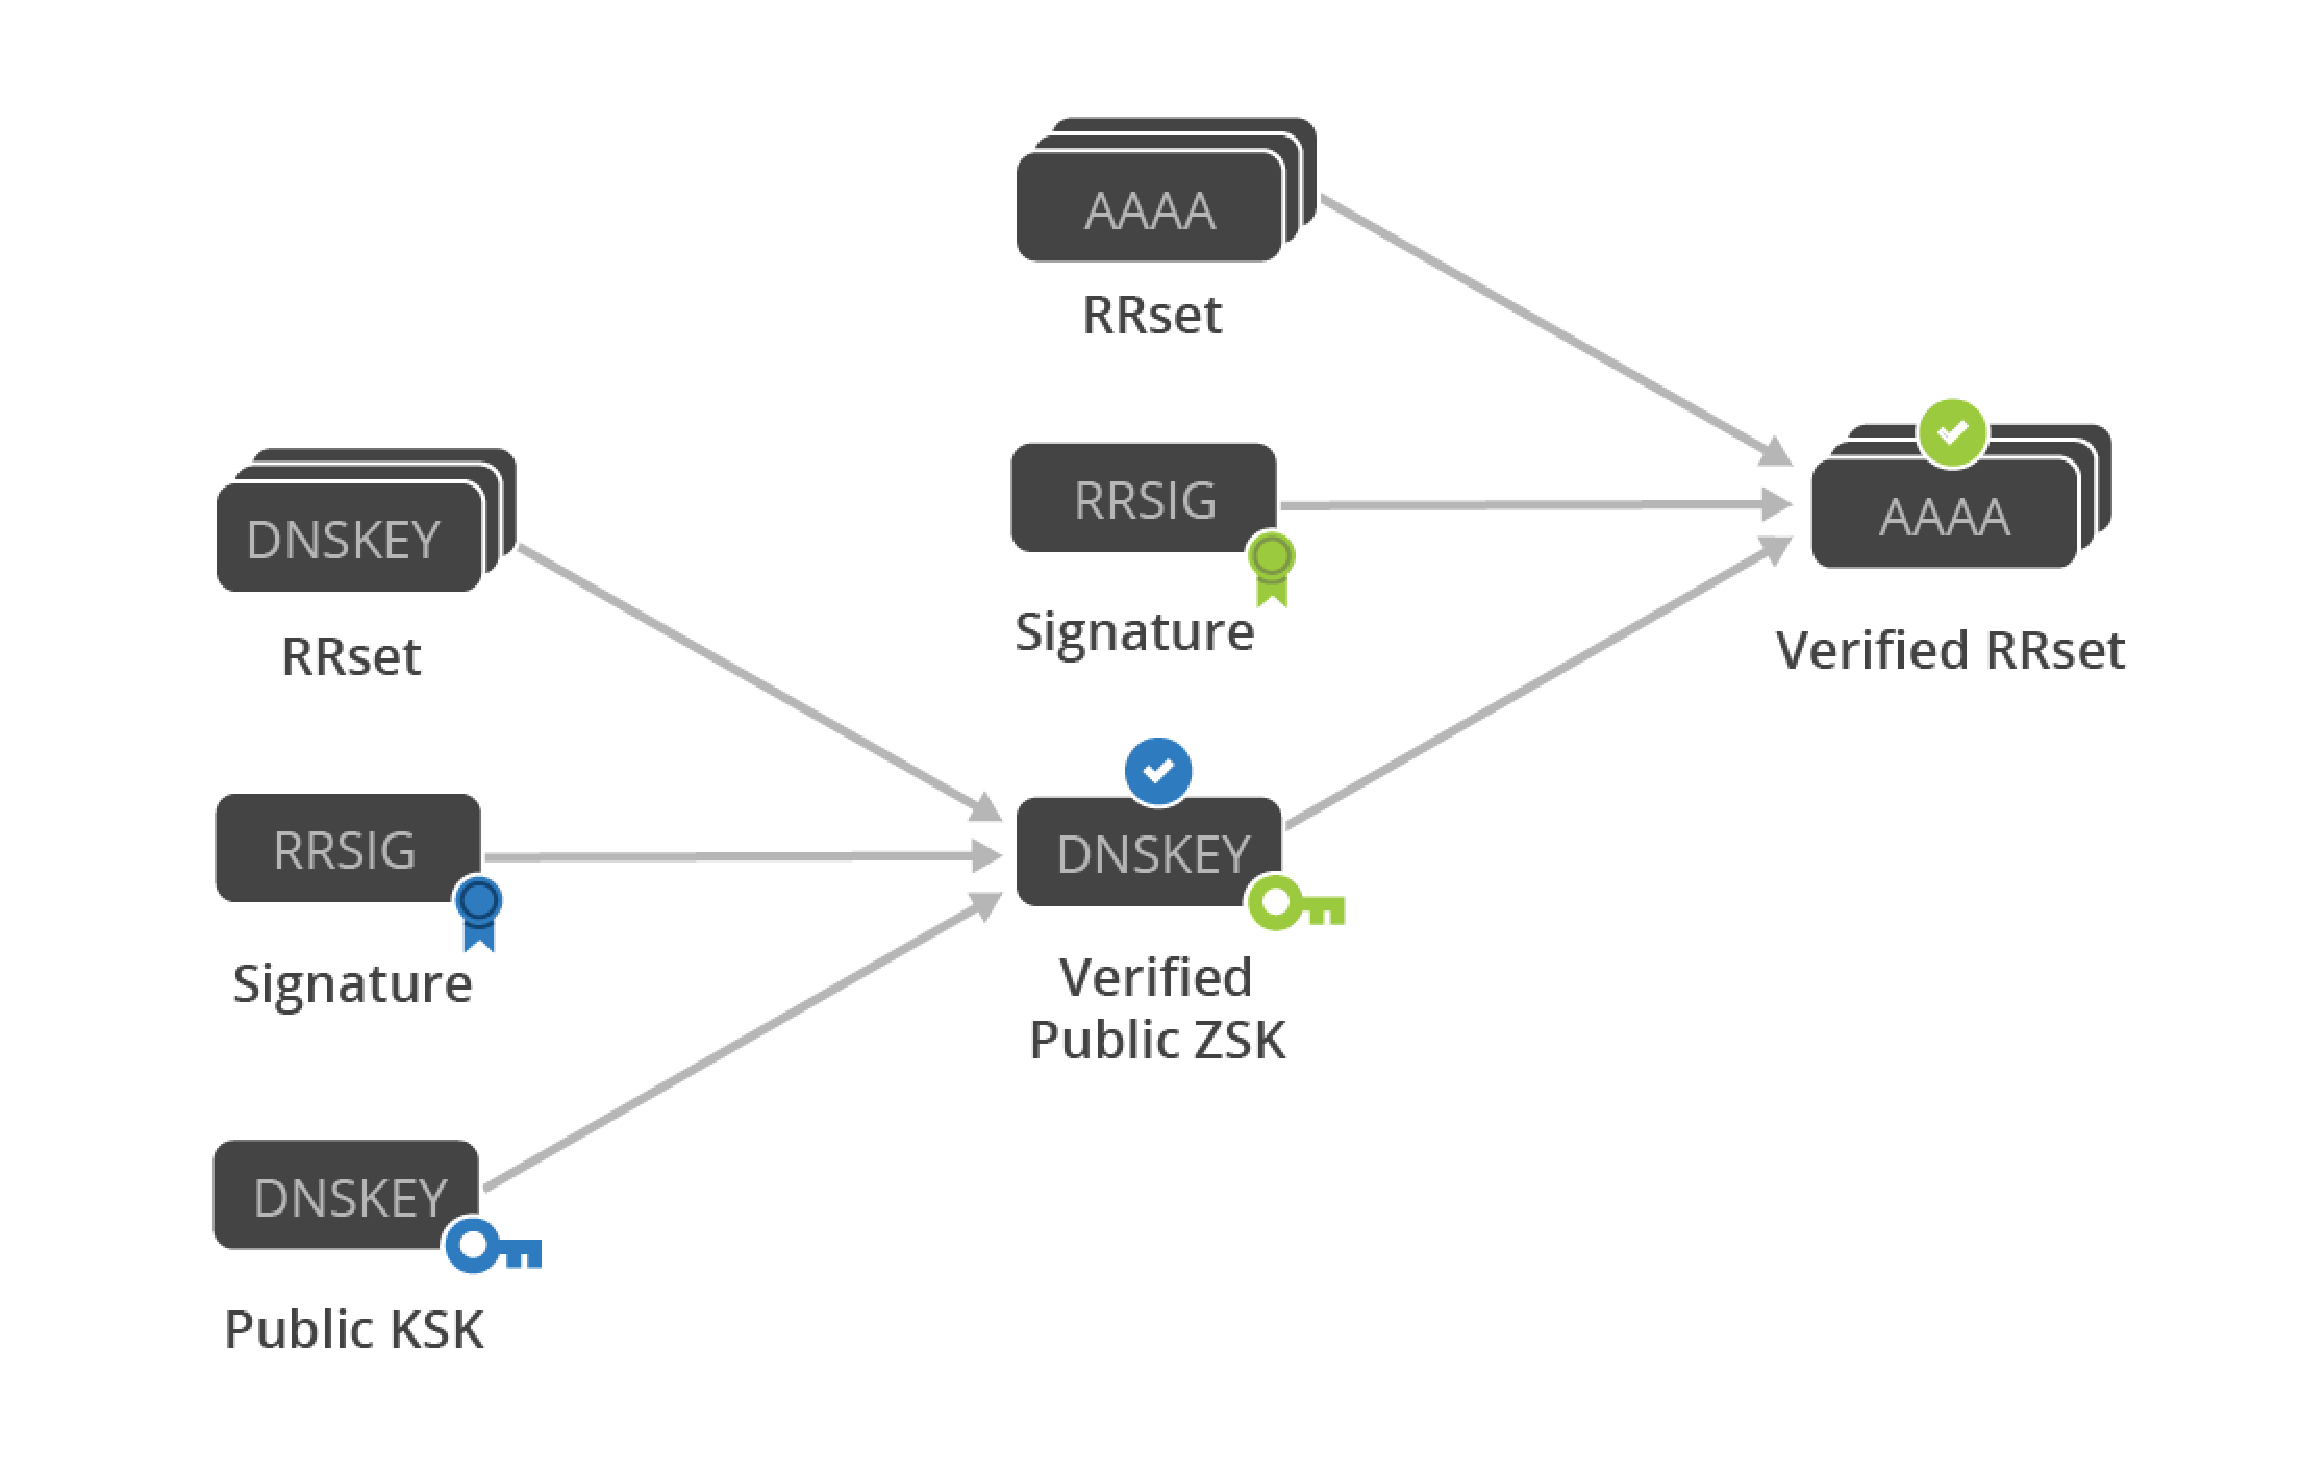
\includegraphics[scale=0.4]{complete_req.eps}
	\caption{Verificação completa da autenticidade do registro.}
	\label{fig:keys}
\end{figure}

Resumidamente, a resolução de nome de forma segura é realizada pelo cliente da seguinte forma:
\begin{itemize}
	\item Solicite o RRset desejado, que também retorna o registro RRSIG correspondente.
	\item Solicite a ZSK e KSK pública, que também retornam o RRSIG para o DNSKEY RRset.
	\item Verifique se o RRSIG do RRset solicitado com a ZSK público.
	\item Verifique se o RRSIG do DNSKEY RRset com o KSK público.
\end{itemize}

É importante ressaltar que o serviço de DNSSEC configurado neste trabalho não provê registro no \textit{delegation signer} (DS) para uma KSK, isso devido ao custo atrelado à aquisição de um registro em servidores autorizados. Entretanto, o processo de configuração do DS foi estudado e pode ser encontrado por completo na \textit{wiki} do projeto no \textit{github}\footnote{documentação sobre configuração do DS: https://github.com/ArthurJahn/FRC-Final/wiki.}.

\chapter{Resultados}

\section{Implementação da Solução}
O ecosistema desenvolvido nesse projeto, tem como base a utilização de máquinas \textit{Vagrant}, que provê serviços de virtualização de ambientes para facilitar configuração de diferentes ambientes para vários sistemas operacionais. O provedor de máquinas virtuais utilizado neste trabalho foi o VirtualBox. Para a configuração do ambiente, é necessário a instalação do vagrant \footnote{Vagrant disponível em: https://www.vagrantup.com/} e do VirtualBox \footnote{VirtualBox disponível em: https://www.virtualbox.org/}.\\

Foram desenvolvidos \textit{scripts} para inicialização das máquinas e configurações dos serviços, todos os passos para subir o ambiente completo foi passado para o script executável \textit{quick-start} que sobe as máquinas e gera um arquivo de \textit{log} para uma requisição a um serviço DNS seguro provido pelo servidor DNS configurado. Todo o ambiente pode ser desligado por meio do \textit{script} de \textit{quick-exit} que destrói os ambientes criados e remove arquivos temporários.\\

Execute os seguintes passos para subir o ambiente: Com as dependências instaladas, execute o arquivo quick-start encontrado na pasta vagrant. Esse executável irá inicializar um servidor DNS seguro configurando a zona \textit{redesfga.com}, uma servidor apache para onde a zona configurada aponta e um cliente que realizará uma requisição de resolução de nome ao servidor DNS. O resultado da requisição é encontrado no arquivo dnssec.log na pasta vagrant, e mostra todo o processo executado para fazer a requisição segura do domínio passado.\\

\section{Considerações}

O DNS é um serviço crucial para o funcionamento da internet atualmente. Entretanto não foi idealizado provendo serviços de segurança, o que gera várias vulnerabilidades que são utilizadas para atacantes gerarem comportamentos idesejados da rede. \\

Com esse trabalho foi possível identificar vulnerabilidades do serviço de DNS, configurar extensões de segurança DNSSEC, verificar os passos para a aquisição de respostas de requisições DNS de forma segura e compreender como os serviços de verificação de autenticidade da internet funcionam e quem é capaz de prover tais serviços. \\

Nesse sentido todos os objetivos propostos foram alcançados e o aprendizado obtido por meio da atividade prática mostrou a complexidade das operações relacionadas ao provimento de serviços seguros na internet.

\end{document}  %Fim do documento
